% GNUPLOT: LaTeX picture with Postscript
\begingroup
  \makeatletter
  \providecommand\color[2][]{%
    \GenericError{(gnuplot) \space\space\space\@spaces}{%
      Package color not loaded in conjunction with
      terminal option `colourtext'%
    }{See the gnuplot documentation for explanation.%
    }{Either use 'blacktext' in gnuplot or load the package
      color.sty in LaTeX.}%
    \renewcommand\color[2][]{}%
  }%
  \providecommand\includegraphics[2][]{%
    \GenericError{(gnuplot) \space\space\space\@spaces}{%
      Package graphicx or graphics not loaded%
    }{See the gnuplot documentation for explanation.%
    }{The gnuplot epslatex terminal needs graphicx.sty or graphics.sty.}%
    \renewcommand\includegraphics[2][]{}%
  }%
  \providecommand\rotatebox[2]{#2}%
  \@ifundefined{ifGPcolor}{%
    \newif\ifGPcolor
    \GPcolorfalse
  }{}%
  \@ifundefined{ifGPblacktext}{%
    \newif\ifGPblacktext
    \GPblacktexttrue
  }{}%
  % define a \g@addto@macro without @ in the name:
  \let\gplgaddtomacro\g@addto@macro
  % define empty templates for all commands taking text:
  \gdef\gplbacktext{}%
  \gdef\gplfronttext{}%
  \makeatother
  \ifGPblacktext
    % no textcolor at all
    \def\colorrgb#1{}%
    \def\colorgray#1{}%
  \else
    % gray or color?
    \ifGPcolor
      \def\colorrgb#1{\color[rgb]{#1}}%
      \def\colorgray#1{\color[gray]{#1}}%
      \expandafter\def\csname LTw\endcsname{\color{white}}%
      \expandafter\def\csname LTb\endcsname{\color{black}}%
      \expandafter\def\csname LTa\endcsname{\color{black}}%
      \expandafter\def\csname LT0\endcsname{\color[rgb]{1,0,0}}%
      \expandafter\def\csname LT1\endcsname{\color[rgb]{0,1,0}}%
      \expandafter\def\csname LT2\endcsname{\color[rgb]{0,0,1}}%
      \expandafter\def\csname LT3\endcsname{\color[rgb]{1,0,1}}%
      \expandafter\def\csname LT4\endcsname{\color[rgb]{0,1,1}}%
      \expandafter\def\csname LT5\endcsname{\color[rgb]{1,1,0}}%
      \expandafter\def\csname LT6\endcsname{\color[rgb]{0,0,0}}%
      \expandafter\def\csname LT7\endcsname{\color[rgb]{1,0.3,0}}%
      \expandafter\def\csname LT8\endcsname{\color[rgb]{0.5,0.5,0.5}}%
    \else
      % gray
      \def\colorrgb#1{\color{black}}%
      \def\colorgray#1{\color[gray]{#1}}%
      \expandafter\def\csname LTw\endcsname{\color{white}}%
      \expandafter\def\csname LTb\endcsname{\color{black}}%
      \expandafter\def\csname LTa\endcsname{\color{black}}%
      \expandafter\def\csname LT0\endcsname{\color{black}}%
      \expandafter\def\csname LT1\endcsname{\color{black}}%
      \expandafter\def\csname LT2\endcsname{\color{black}}%
      \expandafter\def\csname LT3\endcsname{\color{black}}%
      \expandafter\def\csname LT4\endcsname{\color{black}}%
      \expandafter\def\csname LT5\endcsname{\color{black}}%
      \expandafter\def\csname LT6\endcsname{\color{black}}%
      \expandafter\def\csname LT7\endcsname{\color{black}}%
      \expandafter\def\csname LT8\endcsname{\color{black}}%
    \fi
  \fi
    \setlength{\unitlength}{0.0500bp}%
    \ifx\gptboxheight\undefined%
      \newlength{\gptboxheight}%
      \newlength{\gptboxwidth}%
      \newsavebox{\gptboxtext}%
    \fi%
    \setlength{\fboxrule}{0.5pt}%
    \setlength{\fboxsep}{1pt}%
\begin{picture}(5760.00,7200.00)%
    \gplgaddtomacro\gplbacktext{%
      \csname LTb\endcsname%%
      \put(444,5296){\makebox(0,0)[r]{\strut{}0.00e+00}}%
      \csname LTb\endcsname%%
      \put(444,5648){\makebox(0,0)[r]{\strut{}3.00e-09}}%
      \csname LTb\endcsname%%
      \put(444,6000){\makebox(0,0)[r]{\strut{}6.00e-09}}%
      \csname LTb\endcsname%%
      \put(444,6351){\makebox(0,0)[r]{\strut{}9.00e-09}}%
      \csname LTb\endcsname%%
      \put(444,6703){\makebox(0,0)[r]{\strut{}1.20e-08}}%
      \csname LTb\endcsname%%
      \put(1300,4724){\makebox(0,0){\strut{}}}%
      \csname LTb\endcsname%%
      \put(2024,4724){\makebox(0,0){\strut{}}}%
      \csname LTb\endcsname%%
      \put(2748,4724){\makebox(0,0){\strut{}}}%
      \csname LTb\endcsname%%
      \put(3471,4724){\makebox(0,0){\strut{}}}%
      \csname LTb\endcsname%%
      \put(4195,4724){\makebox(0,0){\strut{}}}%
      \csname LTb\endcsname%%
      \put(4919,4724){\makebox(0,0){\strut{}}}%
    }%
    \gplgaddtomacro\gplfronttext{%
      \csname LTb\endcsname%%
      \put(-722,5999){\rotatebox{-270}{\makebox(0,0){\strut{}$\Phi_{\rm weak}(0,r)$}}}%
    }%
    \gplgaddtomacro\gplbacktext{%
      \csname LTb\endcsname%%
      \put(444,3184){\makebox(0,0)[r]{\strut{}0.00e+00}}%
      \csname LTb\endcsname%%
      \put(444,3536){\makebox(0,0)[r]{\strut{}1.50e-08}}%
      \csname LTb\endcsname%%
      \put(444,3888){\makebox(0,0)[r]{\strut{}3.00e-08}}%
      \csname LTb\endcsname%%
      \put(444,4239){\makebox(0,0)[r]{\strut{}4.50e-08}}%
      \csname LTb\endcsname%%
      \put(444,4591){\makebox(0,0)[r]{\strut{}6.00e-08}}%
      \csname LTb\endcsname%%
      \put(1300,2612){\makebox(0,0){\strut{}}}%
      \csname LTb\endcsname%%
      \put(2024,2612){\makebox(0,0){\strut{}}}%
      \csname LTb\endcsname%%
      \put(2748,2612){\makebox(0,0){\strut{}}}%
      \csname LTb\endcsname%%
      \put(3471,2612){\makebox(0,0){\strut{}}}%
      \csname LTb\endcsname%%
      \put(4195,2612){\makebox(0,0){\strut{}}}%
      \csname LTb\endcsname%%
      \put(4919,2612){\makebox(0,0){\strut{}}}%
    }%
    \gplgaddtomacro\gplfronttext{%
      \csname LTb\endcsname%%
      \put(-722,3887){\rotatebox{-270}{\makebox(0,0){\strut{}$\Phi_{\rm inter}(0,r)$}}}%
    }%
    \gplgaddtomacro\gplbacktext{%
      \csname LTb\endcsname%%
      \put(444,1072){\makebox(0,0)[r]{\strut{}0.00e+00}}%
      \csname LTb\endcsname%%
      \put(444,1424){\makebox(0,0)[r]{\strut{}3.00e-08}}%
      \csname LTb\endcsname%%
      \put(444,1776){\makebox(0,0)[r]{\strut{}6.00e-08}}%
      \csname LTb\endcsname%%
      \put(444,2127){\makebox(0,0)[r]{\strut{}9.00e-08}}%
      \csname LTb\endcsname%%
      \put(444,2479){\makebox(0,0)[r]{\strut{}1.20e-07}}%
      \csname LTb\endcsname%%
      \put(1300,500){\makebox(0,0){\strut{}0.0}}%
      \csname LTb\endcsname%%
      \put(2024,500){\makebox(0,0){\strut{}0.2}}%
      \csname LTb\endcsname%%
      \put(2748,500){\makebox(0,0){\strut{}0.4}}%
      \csname LTb\endcsname%%
      \put(3471,500){\makebox(0,0){\strut{}0.6}}%
      \csname LTb\endcsname%%
      \put(4195,500){\makebox(0,0){\strut{}0.8}}%
      \csname LTb\endcsname%%
      \put(4919,500){\makebox(0,0){\strut{}1.0}}%
    }%
    \gplgaddtomacro\gplfronttext{%
      \csname LTb\endcsname%%
      \put(-722,1775){\rotatebox{-270}{\makebox(0,0){\strut{}$\Phi_{\rm strong}(0,r)$}}}%
      \put(3109,170){\makebox(0,0){\strut{}$r$}}%
    }%
    \gplbacktext
    \put(0,0){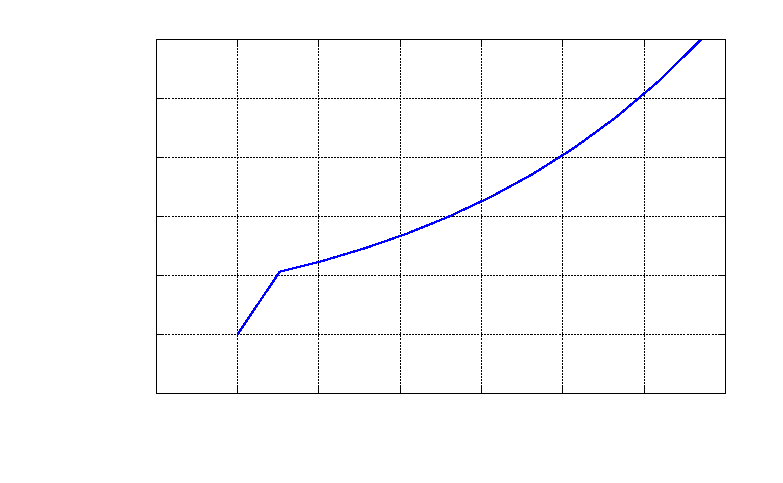
\includegraphics{origin_problem}}%
    \gplfronttext
  \end{picture}%
\endgroup
